\section{Definition}

A Platform-Agnostic Bytecode (PAB), from now on will be defined as a bytecode that follows those two main principles:
\begin{itemize}
    \item Turing Completeness
    \item Support for tooling that makes it executable on every machine
\end{itemize}

A bytecode implementing these principles is ideally designed to be executed on a virtual machine that follows general patterns. This design should make easier the compilation to another real machine's bytecode. Examples of real architectures with specified bytecode are AMD and Intel with x86 or ARM with aarch64. % TODO: check this last sentence

\section{Execution}

PABs require multiple phases of compilation. The first one is encountered when you want to compile your High-Level language to the PAB using a Cross-Compiler. Once you have the PAB code, you should be able to run it on every machine using another compiler that will create the final executable code.

Re-compiling is not the only way to execute a PAB. Another common solution is to implement a Virtual Machine (VM) able to run arbitrary PAB code interpreting it.

\section{Key features}

Every bytecode, ideally, can become a PAB if tools to make it runnable to different machine exist. There are however some metrics to define which one is better than others; example of metrics are:

\begin{description}[style=nextline]
  \item[Hardware Independence]
        If tightly related to specific hardware, a bytecode can't become a PAB because translations to different hardware would be impossible. A weakly coupled bytecode though can become a PAB if the coupling to a specific hardware is negligible and requires some minor adaptations to run on different hardware is required. A  completely hardware independent bytecode, that does not make any specific assumption on the hardware on which will be running on, is the best.
  \item[Sandboxing]
        The machine used to execute the PAB is defined as \textit{embedder}. The embedder will execute arbitrary code, possibly malicious.  A sandboxed environment is the typical solution to overcome any security problem. The execution in a different environment makes it almost impossible to compromise the embedder from the PAB code. Implementing a proper sandboxed environment is embedder dependent but a PAB can be more or less suitable for this feature.

        \begin{figure}[h]
          \centering
          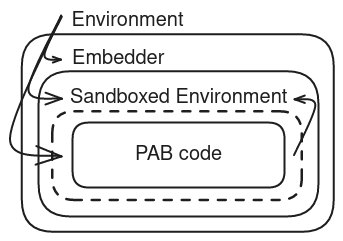
\includegraphics[width=0.4\linewidth]{sandboxed_env.png}
          \caption{Sandboxing graphic example}
          \label{fig:Sandboxing graphic example}
        \end{figure}

  \item[Efficiency]
        The efficiency of a PAB has several facets, it could refer to:

        \begin{itemize}
          \item the efficiency of compiling High-Level Language to the PAB
          \item the efficiency of the execution of the PAB. In this case it could refer to the compilation to the final bytecode and the subsequent execution, the interpretation or more complex solutions
        \end{itemize}

        Generally the first is not really related to the PAB, but more on the used tools (examples gcc, rustc, etc.). The execution efficiency is the real issue: how fast a PAB can be executed on a machine is crucial.
  \item[Tool Simplicity]
        The easiness of compiling a High-Level language and  executing the PAB is very important to make it usable by every one.
  \item[Support as Compilation Target]
        Writing bytecode by hand is something really rare and done only in specific cases. Every compiled language has a compiler to make this, and is very important for a PAB to support the compilation from as many languages as possible.
\end{description}

\section{Current usage}

PAB are already widely used. A few examples are:

\begin{itemize}
  \item
        The Java Virtual Machine (JVM) is one of the first that made the portability of the code one of the main concern of the language
  \item
        % Is the cite useful here?
        Linux brought eBPF~\cite{ebpf}, explained in one of the following chapters, into the kernel, enabling arbitrary programs to be executed in a privileged context (OS level)
  \item
        LLVM IR is the LLVM~\cite{LLVM} assembly language, it provides type safety, low-level operations, flexibility, and the capability of representing ‘all’ high-level languages cleanly. It is the common code representation used throughout all phases of the LLVM compilation strategy.
  \item
        WebAssembly~\cite{wasm-core-spec} is a safe, portable, low-level code format designed for efficient execution and compact representation.
\end{itemize}

\section{PAB in blockchains}

Blockchains are distributed systems that need to agree on the execution of arbitrary code performed on different machines. While it is not the purpose of this work to provide a detailed explanation of blockchains, it is essential for our purposes to understand that the goal of each machine is to produce blocks that are connected with hashes to the previous blocks, so creating a block chain. Machines that take part in the block production are also called nodes, and they are part of a trust-less network. This means that nodes can't simply trust other nodes and rely on the blocks produced by them, on the contrary they must verify in some way the correctness of those blocks by themselves.

Let's simplify and define the block production algorithm as a function that takes an arbitrary input and produces and arbitrary output. Input and output are then bundled together to produce a block (little caveat, though, is that each input depends also on all the previous produced blocks).

If Block A is the first block, it contains A.input and A.output (A.input is a special input that does not depend on the previous block because A is the genesis block). A node then produces block B on top of block A while another node produces block C on top of A. At this point the new blocks can be arbitrarily added on top of either A, B, or C. A new node that just joins the network must decide where to append a new block, Figure~\ref{fig:block_prod}.  This question is extremely complex and outside our scope. We will however provide an answer to a part of the question: on top of which block the node must not attach the new block.

\begin{figure}[h]
  \centering
  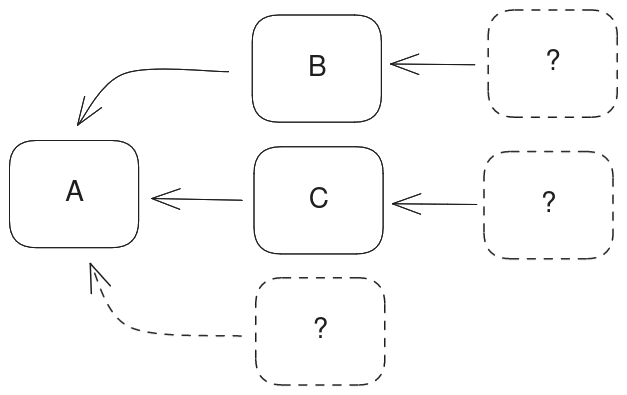
\includegraphics[width=0.5\linewidth]{block_prod.png}
  \caption{Block Production Example}
  \label{fig:block_prod}
\end{figure}

PABs are the answer to this question. The main point of having input and output contained in the blocks, inside a trust-less network, is to let the nodes re-validate blocks to make sure other nodes behaved correctly.

The function that gives the output must return the same result regardless of the node and the node's architecture to make everyone agree on the correctness of new blocks. This property is  called `execution determinism`.

The new node in the network will validate all the blocks in the chain. It will start from the block A,  re-compute A.output starting from A.input, make sure the block is correct (i.e., compare the computed A.output with the A.output contained in the block). The new node will then repeat the process for each block up in the chain until the leafs. Every invalid block will be discarded as a possible base on which to append a new block.

\

PABs are the most suitable solution to implement this validation. PABs can encode any type of logic (first principle of a PAB) and can be executed on every machine (second principle). PABs can also fully address execution determinism, as we will describe in the following chapters.
